\documentclass{article}

\usepackage{graphicx}
\usepackage{tikz}
\usepackage{tikzsymbols}
\usetikzlibrary{calc,patterns,shapes.geometric}
\pagestyle{empty}
\usepackage[margin=0pt]{geometry}
\geometry{papersize={14in,12in}}

\def\centerarc[#1](#2)(#3:#4:#5){\draw[#1] ($(#2)+({#5*cos(#3)},{#5*sin(#3)})$) arc (#3:#4:#5);}

\begin{document}
	\begin{figure}
		\centering
		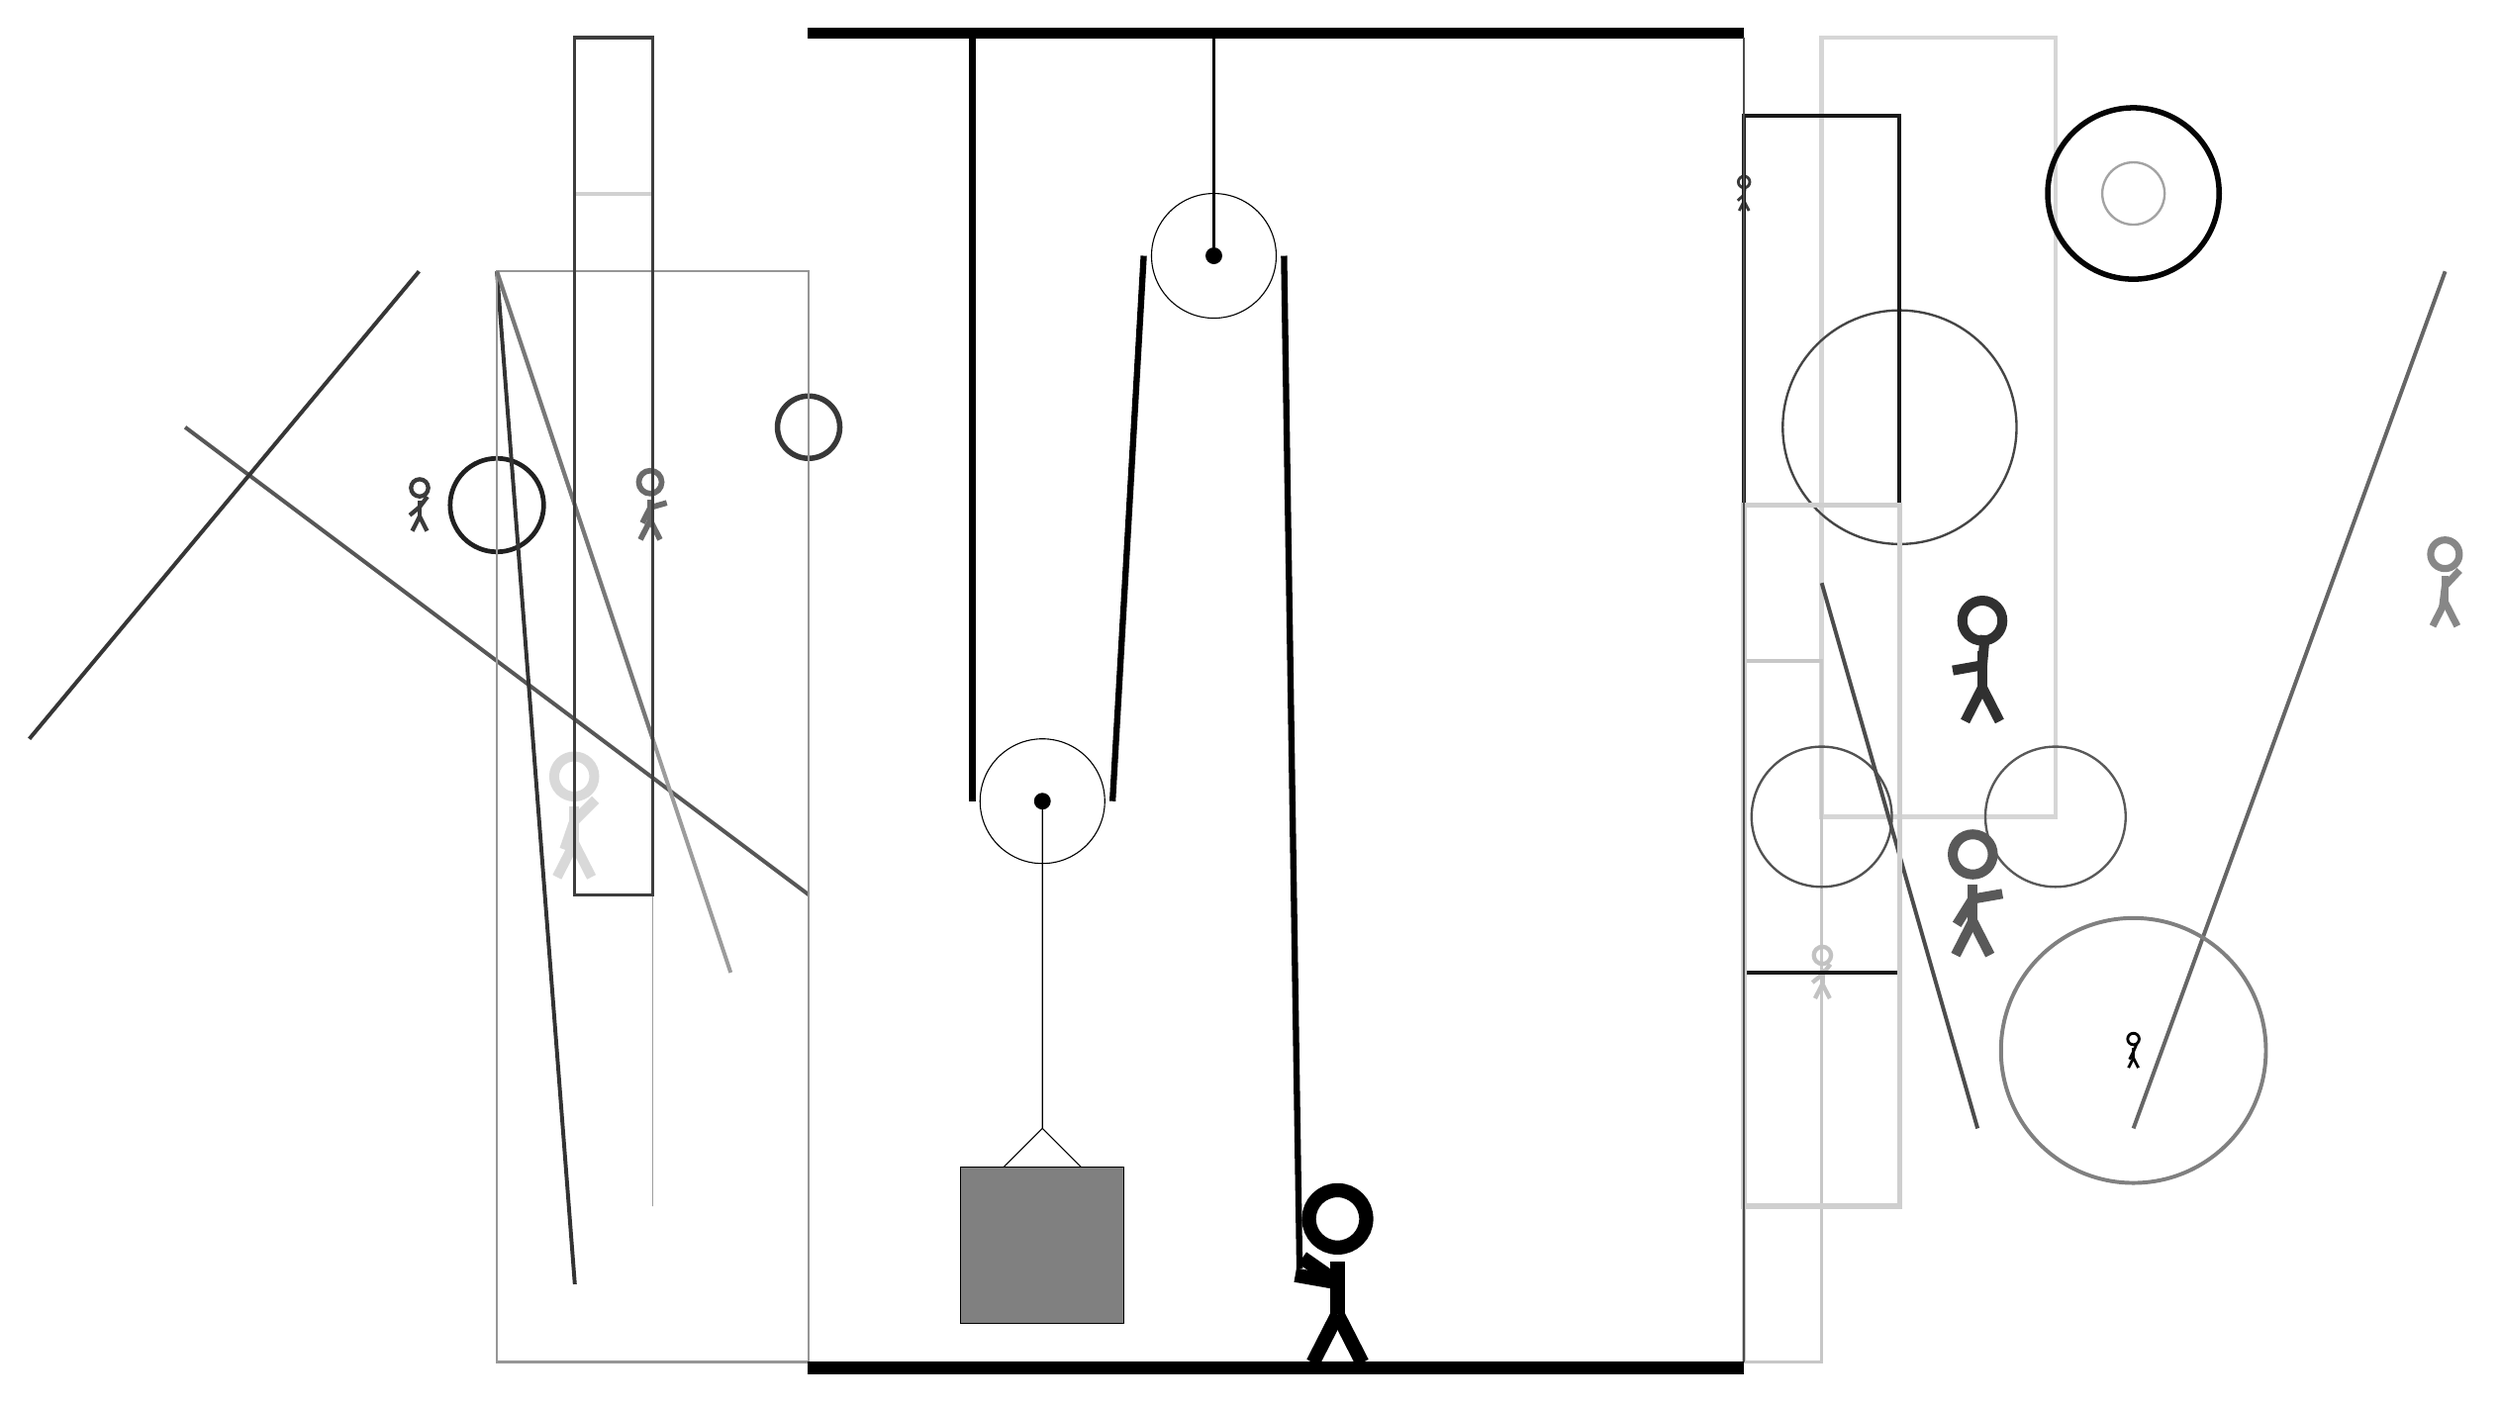
\begin{tikzpicture}
			%%%%% START %%%%%
			
			\draw[fill=black] (-2, 14) rectangle (10, 14.125);
			
			\draw (3.2, 11.2) circle (0.8);
			\draw[fill=black] (3.2, 11.2) circle (0.1);
			\draw[thick] (3.2, 11.2) -- (3.2, 14);
			
			\draw (1, 4.2) circle (0.8);
			\draw[fill=black] (1, 4.2) circle (0.1);
			
			\draw (1, 4.2) -- (1, 0) -- (0.5, -0.5);
			\draw (1, 0) -- (1.5, -0.5);
			\draw[fill=black!50] (-0.05, -0.5) rectangle (2.05, -2.5);
			
			\draw[line width=0.8mm] (0.1, 14) -- (0.1, 4.2);
			\centerarc[line width=0.8mm](1, 4.2)(180:360:0.9);
			\draw[line width=0.8mm](1.9, 4.2) -- (2.3, 11.2);
			\centerarc[line width=0.8mm](3.2, 11.2)(0:180:0.9);
			\draw[line width=0.8mm](4.1, 11.2) -- (4.3, -1.8);
			
			\draw[line width=0.6mm, color=black!16] (11, 14) rectangle (14, 4);
			
			\draw [line width=0.3mm, color=black!73](12, 9) circle (1.5);
			\draw[line width=0.5mm, color=black!66](-2, 3) -- (-10, 9);
			\draw [line width=0.7mm, color=black!78](-2, 9) circle (0.4);
			
			\draw[line width=0.4mm, color=black!22] (11, 6) rectangle (10, -3);
			\node[line width=0.7mm, color=black!24] at (11, 2) {\Strichmaxerl[3][39][52]};
			\draw [line width=0.6mm, color=black!87](-6, 8) circle (0.6);
			
			\draw[line width=0.5mm, color=black!39](-3, 2) -- (-6, 11);
			\node[line width=0.2mm, color=black!65] at (13, 3) {\Strichmaxerl[7][58][10]};
			\draw [line width=0.7mm, color=black!98](15, 12) circle (1.1);
			\node[line width=0.4mm, color=black!77] at (10, 12) {\Strichmaxerl[2][43][82]};
			\draw[line width=0.5mm, color=black!80](-6, 11) -- (-5, -2);
			\node[line width=0.7mm, color=black!15] at (-5, 4) {\Strichmaxerl[7][71][45]};
			
			\draw[line width=0.3mm, color=black!41] (-2, 11) rectangle (-6, -3);
			\draw [line width=0.3mm, color=black!68](11, 4) circle (0.9);
			\draw[line width=0.5mm, color=black!90] (10, 13) rectangle (12, 2);
			
			\node[line width=0.5mm, color=black!58] at (-4, 8) {\Strichmaxerl[4][63][16]};
			\draw [line width=0.3mm, color=black!36](15, 12) circle (0.4);
			\draw[line width=0.5mm, color=black!18](-5, 12) -- (-4, 12);
			
			\draw[line width=0.5mm, color=black!79](-7, 11) -- (-12, 5);
			\draw[line width=0.5mm, color=black!53](-6, 11) -- (-4, 5);
			
			\draw[line width=0.5mm, color=black!60](15, 0) -- (19, 11);
			\node[line width=0.7mm, color=black!81] at (13, 6) {\Strichmaxerl[7][10][85]};
			\node[line width=0.7mm, color=black!77] at (-7, 8) {\Strichmaxerl[3][40][53]};
			\draw[line width=0.5mm, color=black!70](13, 0) -- (11, 7);
			\node[line width=0.2mm, color=black!98] at (15, 1) {\Strichmaxerl[2][63][68]};
			\draw[line width=0.7mm, color=black!19] (10, -1) rectangle (12, 8);
			\draw [line width=0.5mm, color=black!50](15, 1) circle (1.7);
			\node[line width=0.2mm, color=black!47] at (19, 7) {\Strichmaxerl[5][83][47]};
			
			\draw[line width=0.3mm, color=black!70] (10, -3) rectangle (10, 14);
			\draw[line width=0.2mm, color=black!38] (-4, 4) rectangle (-4, -1);
			
			\draw [line width=0.3mm, color=black!65](14, 4) circle (0.9);
			\draw[line width=0.4mm, color=black!76] (-4, 14) rectangle (-5, 3);
			
			\node at (4.7, -1.9) {\Strichmaxerl[10][-35][170]};
			
			\draw[fill=black] (-2, -3) rectangle (10, -3.15);
			
			%%%%% END %%%%%
		\end{tikzpicture}
	\end{figure}	
\end{document}